\begin{center}

\begin{tikzpicture}[font=\small,overlay,
mycirclex/.style={draw, circle, minimum size=1.0em, inner sep = 0.2mm}, 
mydiamond/.style={draw, diamond, minimum size=0.78em, inner sep = 0mm}, 
myrectang/.style={rounded corners, draw, rectangle, minimum size=0.60em, inner sep = 0.8mm, line width = 0.03cm}, 
>=stealth]

\definecolor{mygreen}{rgb}{0, 0.7, 0}
\definecolor{myyellow}{rgb}{0.8, 0.6, 0}

\def\colx{black}
\def\cola{red} 
\def\colb{blue}
\def\colc{violet}
\def\cold{cyan} 
\def\cole{myyellow}
\def\colf{brown}


\def\len{1.6cm}

% G1
\begin{scope}[local bounding box=bbox, xshift=-6.4cm]
\path<2-> node[mycirclex] (v1) at (1.0 * \len, 0) {$s$};
\path<2-> node[mycirclex] (v2) at (2.0 * \len, 0) {$a$};
\path<2-> node[mycirclex] (v3) at (3.0 * \len, 0) {$b$};
\path<2-> node[mycirclex] (v4) at (4.0 * \len, 0) {$c$};
\path<2-> node[mycirclex] (v5) at (5.0 * \len, 0) {$d$};
\path<2-> node[mycirclex] (v6) at (6.0 * \len, 0) {$t$};

\path<3-> [draw, \cola, ->, line width=0.09cm, bend left = 40] (v1) to (v3);
\path<3-> [draw, \cola, ->, line width=0.09cm] (v3) -- (v4);
\path<3-> [draw, \cola, ->, line width=0.09cm] (v4) -- (v5);
\path<3-> [draw, \cola, ->, line width=0.09cm] (v5) -- (v6);
\path<3-> node[myrectang, rounded corners, \cola] at (6.8 * \len, 0) {$a(P_1) = 4$};

\path<2-> [draw, \colx, ->, line width=0.04cm] (v1) -- (v2);
\path<2-> [draw, \colx, ->, line width=0.04cm] (v2) -- (v3);
\path<2-> [draw, \colx, ->, line width=0.04cm] (v3) -- (v4);
\path<2-> [draw, \colx, ->, line width=0.04cm] (v4) -- (v5);
\path<2-> [draw, \colx, ->, line width=0.04cm] (v5) -- (v6);

\path<2-> [draw, \colx, ->, line width=0.04cm, bend left = 40] (v1) to (v3);
\path<2-> [draw, \colx, ->, line width=0.04cm, bend left = 40] (v3) to (v5);
\path<2-> [draw, \colx, ->, line width=0.04cm, bend left =-27] (v2) to (v5);
\path<2-> [draw, \colx, ->, line width=0.04cm, bend left =-40] (v4) to (v6);

\path<2-> node at (1.5 * \len, 0.2cm) {$4$};
\path<2-> node at (2.5 * \len, 0.2cm) {$1$};
\path<2-> node at (3.5 * \len, 0.2cm) {$5$};
\path<2-> node at (4.5 * \len, 0.2cm) {$4$};
\path<2-> node at (5.5 * \len, 0.2cm) {$9$};

\path<2-> node at (2.0 * \len, 0.85cm) {$6$};
\path<2-> node at (4.0 * \len, 0.85cm) {$2$};
\path<2-> node at (5.0 * \len,-0.85cm) {$1$};
\path<2-> node at (3.5 * \len,-0.85cm) {$3$};

\path<4-> [draw, \colx, ->, line width=0.1cm] (3.5 * \len, -1.2cm) -- (3.5 * \len, -1.8cm);

\end{scope}

%\path<2-> [draw, rounded corners] ($(bbox.south west) - (0.00cm, 0.25cm)$) rectangle ($(bbox.north east) + (0.1cm, 0)$);
%\node at ($(bbox.south) - (0.00cm, 0.2cm)$) [label=below:{$G_2 - G_1 = \{c\}$}]{};


% G2
\begin{scope}[local bounding box=bbox, xshift=-6.4cm, yshift = -2.6cm]
\path<4-> node[mycirclex] (v1) at (1.0 * \len, 0) {$s$};
\path<4-> node[mycirclex] (v2) at (2.0 * \len, 0) {$a$};
\path<4-> node[mycirclex] (v3) at (3.0 * \len, 0) {$b$};
\path<4-> node[mycirclex] (v4) at (4.0 * \len, 0) {$c$};
\path<4-> node[mycirclex] (v5) at (5.0 * \len, 0) {$d$};
\path<4-> node[mycirclex] (v6) at (6.0 * \len, 0) {$t$};

\path<5-> [draw, \colb, ->, line width=0.09cm] (v1) -- (v2);
\path<5-> [draw, \colb, ->, line width=0.09cm, bend left =-27] (v2) to (v5);
\path<5-> [draw, \colb, ->, line width=0.09cm] (v5) -- (v6);
\path<5-> node[myrectang, rounded corners, \colb] at (6.8 * \len, 0) {$a(P_2) = 3$};

\path<4-> [draw, \colx, ->, line width=0.04cm] (v1) -- (v2);
\path<4-> [draw, \colx, ->, line width=0.04cm] (v2) -- (v3);
\path<4-> [draw, \colx, ->, line width=0.04cm] (v3) -- (v4);
\path<4-> [draw, \colx, ->, line width=0.04cm] (v5) -- (v6);

\path<4-> [draw, \colx, ->, line width=0.04cm, bend left = 40] (v1) to (v3);
\path<4-> [draw, \colx, ->, line width=0.04cm, bend left = 40] (v3) to (v5);
\path<4-> [draw, \colx, ->, line width=0.04cm, bend left =-27] (v2) to (v5);
\path<4-> [draw, \colx, ->, line width=0.04cm, bend left =-40] (v4) to (v6);

\path<4-> node at (1.5 * \len, 0.2cm) {$4$};
\path<4-> node at (2.5 * \len, 0.2cm) {$1$};
\path<4-> node at (3.5 * \len, 0.2cm) {$1$};
\path<4-> node at (5.5 * \len, 0.2cm) {$5$};

\path<4-> node at (2.0 * \len, 0.85cm) {$2$};
\path<4-> node at (4.0 * \len, 0.85cm) {$2$};
\path<4-> node at (5.0 * \len,-0.85cm) {$1$};
\path<4-> node at (3.5 * \len,-0.85cm) {$3$};
\end{scope}


\end{tikzpicture}
\end{center}
